\chapter{Views}
\section{Logical View}

\begin{figure}[h]
	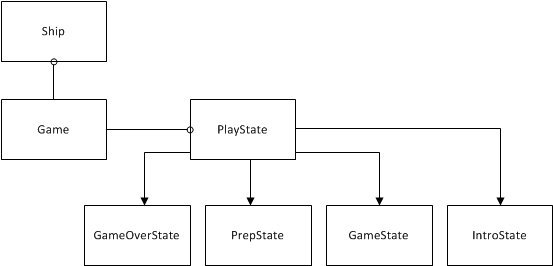
\includegraphics[width=\textwidth]{LogicalView.png}
	\caption{Logical View}
	\label{fig:LogicalView}
\end{figure}

The diagram shows a simplified overview of the different classes, usages and inheritation. Notation is based on the Logical View notation by Kructhen.\cite{kruchten} 
\\
\texttt{GameOverState}, \texttt{PrepState}, \texttt{GameState} and \texttt{IntroState} all extend a common \texttt{PlayState} class. The main \texttt{Game} class functions as a controller, and controls the state stack. \texttt{Ship} object is used by the main \texttt{Game} class, which instantiates the different ship types with a given set of attributes.
\\
Several more states and objects are discussed earlier in this report, and are not represented in this diagram. The main reason for this descision is to keep the diagram simple and easy to read, the ignored features are either redundant or too specific. 

\section{Development View}
\begin{figure}[h]
	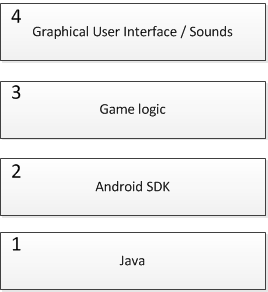
\includegraphics[width=\textwidth]{DevelopmentView.png}
	\caption{Development View}
	\label{fig:DevelopmentView}
\end{figure}

write something smart here

\section{Process View}
something something